\documentclass[a4paper,12pt]{article}
\usepackage[czech]{babel}
\usepackage{graphicx}
\usepackage{geometry}
\geometry{a4paper, margin=1in}


% Packages
\usepackage{amsmath}
\usepackage{graphicx}
\usepackage{float}
\usepackage{longtable}
\usepackage{hyperref}
\usepackage{url}
\usepackage{setspace}
\onehalfspacing
\setlength{\parindent}{0pt}  % No paragraph indentation
\setlength{\parskip}{1em}    % Space between paragraphs

\usepackage[backend=biber,style=authoryear]{biblatex}
\addbibresource{zdroje.bib}

\begin{document}

\begin{titlepage}
    \begin{center}
        {\huge \bfseries Algoritmy počítačové kartografie}\\
        \vspace{3.5em}
        {\Large \bfseries Úloha 2} \\
        \vspace{0.5em}
        {\Large \bfseries Generalizace budov LOD0} \\
        \vspace{3.5em}
        {\large František Macek, Josef Zátka} \\
        \vspace{2.5em}
        
\includegraphics[width=10cm]{logo.png}\\
        \vspace{-2em}
        { \bfseries Univerzita Karlova}\\
        \vspace{0.33em}
        { \bfseries Přírodovědecká fakulta}\\
        \vspace{0.33em}
        { \bfseries Katedra aplikované geoinformatiky a kartografie}\\
        \vspace{10em}
        {\large Praha, 2025}
    \end{center}
\end{titlepage}

\section{Zadání}

\textbf{Úloha č. 2: Generalizace budov LOD0}

\textit{Vstup:} množina budov $B = \{B_i\}_{i=1}^{n}$, \quad budova $B_i = \{P_{i,j}\}_{j=1}^{m}$.

\textit{Výstup:} $G(B_i)$.

Ze souboru načtěte vstupní data představovaná lomovými body budov a proveďte generalizaci budov do úrovně detailu LOD0. Pro tyto účely použijte vhodnou datovou sadu, např. ZABAGED, testování proveďte nad třemi datovými sadami (historické centrum města, sídliště, izolovaná zástavba).

Pro každou budovu určete její hlavní směry metodami:

\begin{itemize}
    \item Minimum Area Enclosing Rectangle,
    \item PCA.
\end{itemize}

U první metody použijte některý z algoritmů pro konstrukci konvexní obálky. Budovu při generalizaci do úrovně LOD0 nahraďte obdélníkem orientovaným v obou hlavních směrech, se středem v těžišti budovy, jehož plocha bude stejná jako plocha budovy. Výsledky generalizace vhodně vizualizujte.

Otestujte a porovnejte efektivitu obou metod s využitím hodnotících kritérií. Pokuste se rozhodnout, pro které tvary budov dávají metody nevhodné výsledky, a pro které naopak poskytují vhodnou aproximaci.

\section{Údaje o bonusových úlohách}

\begin{small}
\begin{longtable}{|p{12cm}|c|}
    \hline
    \textbf{Krok} & \textbf{Hodnocení} \\
    \hline
    \endfirsthead

    \hline
    \textbf{Krok} & \textbf{Hodnocení} \\
    \hline
    \endhead

    Generalizace budov metodami Minimum Area Enclosing Rectangle a PCA. & 15b \\
    \hline
    \textit{Generalizace budov metodou Longest Edge.} & +5b \\
    \hline
    Generalizace budov metodou Wall Average. & +8b \\
    \hline
    Generalizace budov metodou Weighted Bisector. & +10b \\
    \hline
    Ošetření singulárních případů při konstrukci konvexní obálky. & +2b \\
    \hline
    Načtení vstupních dat ze *.shp. & +10b \\
    \hline
    \textbf{Celkem splněno bodů:} & \textbf{50b} \\
    \hline
\end{longtable}
\end{small}



\section{Úvod}
Kartografická generalizace je proces, při kterém se objekty v mapě zjednodušují tak, aby byly vhodné pro menší měřítko mapy. Jejím cílem je zachovat důležité charakteristiky objektů (polohu, proporce, orientaci), ale potlačit detaily, které by v daném měřítku zbytečně komplikovaly čtení mapy, nebo by vůbec nebyly viditelné.

V této úloze se zaměřujeme na generalizaci půdorysů budov do úrovně detailu LOD0, kdy se původní půdorys budovy nahrazuje zjednodušeným obdélníkem stejné plochy a orientace. Vytvořený obdélník musí zachovat základní charakteristiky původní budovy, především její polohu, plochu a celkovou orientaci.

Při generalizaci budov je klíčové nalézt jejich hlavní směry, které lze určit mnoha metodami. V této práci byly implementovány metody \textbf{Minimum Area Enclosing Rectangle} (též nazývaná Minimum Bounding Rectangle), \textbf{PCA} (Principal Component Analysis), \textbf{Longest Edge}, \textbf{Wall Average} a \textbf{Weighted Bisector}. Každá z nich nabízí jiný přístup k určování hlavních směrů, a tedy i jiný finální výsledek zjednodušeného půdorysu budovy.

Metody byly testovány na různých typech zástavby (historické centrum města, sídliště, izolovaná zástavba), každá z metod je totiž vhodnější pro jiný typ zástavby. Polygony budov byly importovány ze souboru formátu *.shp, jako zdroj byla využita ZABAGED.

V dalších částech zprávy se zaměříme na popis jednotlivých implementovaných algoritmů a vyhodnocení jejich výsledků nad různými typy zástavby. Pro většinu z nich je nezbytná ntaké konstrukce konvexní obálky, první kapitola se tedy zaměří právě na ni.




\section{Konvexní obálka a algoritmus Jarvis Scan}
Konvexní obálka (anglicky convex hull) je nejmenší konvexní polygon, který obsahuje všechny body dané množiny. V kontextu této úlohy slouží konvexní obálka jako vstup pro metodu Minimum Area Enclosing Rectangle – protože minimální opsaný obdélník vždy závisí pouze na bodech tvořících konvexní obvod polygonu \parencite{bayer_prednaska}. Použitím konvexní obálky tak omezíme množství bodů, se kterými dále pracujeme.

Pro výpočet konvexní obálky jsme implementovali algoritmus \textbf{Jarvis Scan}. Jeho princip spočívá v tom, že obal postupně „omotáváme“ kolem množiny bodů. Začínáme bodem s nejnižší x-ovou (v případě shody i y-ovou) souřadnicí, a poté hledáme takový bod, který spolu s aktuálním bodem a libovolným dalším bodem svírá nejmenší kladný úhel. Tento proces se opakuje, dokud se nevrátíme na výchozí bod.

Výhoda Jarvis Scanu spočívá v jednoduché implementaci a intuitivním principu, nevýhodou je jeho časová složitost. V našem případě je však tato složitost vzhledem k omezenému množství vrcholů polygonu nepředstavuje reálný problém.

\begin{figure}[H]
    \centering
    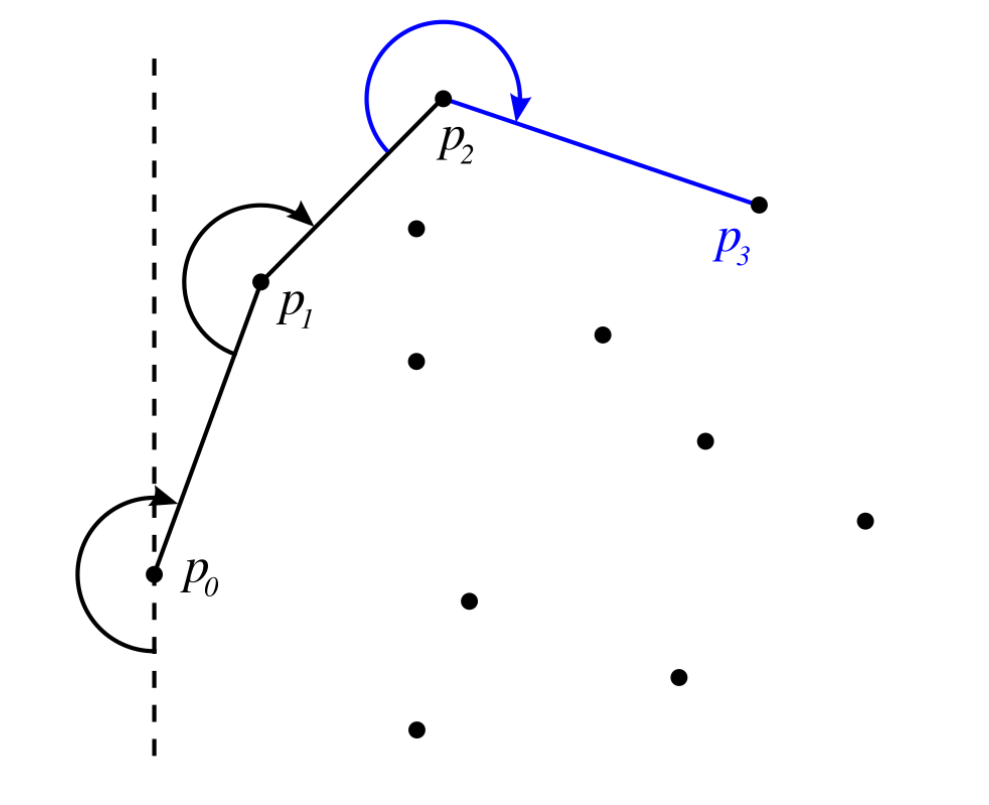
\includegraphics[width=0.6\textwidth]{jarscan.png}
    \caption{Princip konstrukce konvexní obálky pomocí algoritmu Jarvis Scan \parencite{wikimedia_jarvis}}
    \label{fig:jarvis_scan}
\end{figure}

V naší implementaci (funkce \texttt{createCH} v souboru \texttt{algorithms.py}) postupujeme následovně:
\begin{enumerate}
    \item Vyhledáme bod s nejnižší x-ovou souřadnicí (v případě shody ten s nižší y-ovou).
    \item Postupně hledáme takový bod, který tvoří s aktuálním bodem a každým dalším bodem největší kladný orientovaný úhel (pomocí vektorového součinu).
    \item Přidáme tento bod do seznamu výsledné obálky.
    \item Opakujeme, dokud se nevrátíme do výchozího bodu.
\end{enumerate}

Výsledkem je seznam bodů uspořádaných proti směru hodinových ručiček, tvořících konvexní obálku vstupního polygonu.


\section{Minimum Area Enclosing Rectangle}
Minimum Area Enclosing Rectangle (nazývaná také Minimum Bounding Rectangle) je metoda, která pro danou množinu bodů hledá obdélník s nejmenší možnou plochou, který ohraničuje každý bod z této množiny.
Nejprve je vytvořena konvexní obálka. Následně je pro každou svou hranu konvexní obálka natočena tak, aby byla tato hrana rovnoběžná s osou x. Pak se vyhledá minimální a maximální souřadnice x a y (v takto natočené rovině), čímž vznikne minmax box daného natočení. Při procházení všech hran se sleduje, kdy je nalezen obdélník s nejmenší plochou, a ten je pak natočen zpět do původního orientačního systému. 

V naší implementaci je tento postup obsažen ve funkci createMBR (soubor algorithms.py). Metoda využívá následující kroky:

\begin{enumerate}
    \item \textbf{Konstrukce konvexní obálky} pomocí funkce createCH (Jarvis Scan).
    \item \textbf{Opakovaná rotace konvexní obálky} dle orientace jejích hran. Pro hranu, která má směrnici sigma, se polygon pomocí funkce rotate natočí o úhel -sigma tak, aby daná hrana ležela rovnoběžně s osou x.
    \item \textbf{Určení minmax boxu} rotované konvechní obálky. Pomocí createMMB se nalezne nejmenší a největší souřadnice x a y, čímž se definuje obdélník a vypočte se jeho plocha.
    \item \textbf{Uložení minima} je-li plocha nového minmax boxu menší než dosud známá, aktualizuje se a zapamatují se příslušné hodnoty (úhel sigma a plocha).
    \item \textbf{Natočení výsledného obdélníku zpět} o úhel sigma a finální uložení polygonu. 
    \item \textbf{Upravení velikosti} tak, aby výsledný obdélník měl shodnou plochu jako původní budova. K tomu slouží funkce resizeRectangle, která od středu obdélníka proporčně změní velikost stran tak, aby se jeho obsah rovnal obsahu původní budovy.
\end{enumerate}

Postup lze zjednodušeně shrnout v následujícím pseudokódu:

\begin{verbatim}
// Minimum Area Enclosing Rectangle
// Vstup: polygon B (půdorys budovy)
// Výstup: obdélník R minimální možné plochy, 
// natočený a upravený na stejnou plochu jako B

1. Vytvoř konvexní obálku CH z polygonu B:
   CH = createCH(B)

2. Získej první minmax box a jeho plochu:
   (mmb_min, area_min) = createMMB(CH)
   sigma_min = 0

3. Urči n = počet vrcholů CH.

4. Pro každou hranu CH[i], CH[i+1]:
   a) Spočti její úhel:
      dx = CH[i+1].x - CH[i].x
      dy = CH[i+1].y - CH[i].y
      sigma = atan2(dy, dx)
   b) Otoč polygon CH o -sigma:
      ch_r = rotate(CH, -sigma)
   c) Vypočti bounding box a jeho plochu:
      (mmb, area) = createMMB(ch_r)
   d) Pokud area < area_min:
      area_min = area
      mmb_min = mmb
      sigma_min = sigma

5. Uprav výsledný obdélník na plochu původního polygonu B:
   mmb_min_res = resizeRectangle(B, mmb_min)

6. Otoč mmb_min_res zpět o sigma_min:
   R = rotate(mmb_min_res, sigma_min)
\end{verbatim}


\section{Principal Component Analysis (PCA)}
Další implementovanou metodou pro určení hlavních směrů budovy je PCA (Principal Component Analysis). Tato metoda pochází z oblasti statistiky a lineární algebry a slouží k nalezení hlavních os rozptylu dat. V kontextu generalizace budov nám PCA umožňuje určit dominantní směr (obrázek 2), ve kterém jsou body polygonu nejvíce rozprostřeny. Tento směr lze pak využít pro orientaci výsledného obdélníku.

\begin{figure}[H]
    \centering
    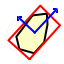
\includegraphics[width=0.6\textwidth]{pca.png}
    \caption{Hlavní směry budovy nalezené metodou PCA \parencite{bayer_prednaska}}
    \label{fig:pca} 
\end{figure}

Postup výpočtu spočívá v tom, že se všechny body polygonu převedou na vektory relativní k těžišti polygonu. Z těchto vektorů se sestaví kovarianční matice, pro kterou se následně vypočítají vlastní vektory a vlastní čísla. Směr s největším vlastním číslem pak odpovídá hlavnímu směru budovy. Druhý vlastní vektor je na tento směr kolmý.

V naší implementaci (funkce \texttt{createBRPCA} v souboru \texttt{algorithms.py}) je postup následující:
\begin{enumerate}
    \item Vypočítáme těžiště polygonu.
    \item Od každého bodu polygonu odečteme souřadnice těžiště a sestavíme matici relativních bodů.
    \item Provedeme dekompozici metodou SVD (Singular Value Decomposition), čímž získáme hlavní směr (první vlastní vektor).
    \item Vypočítáme minmax box polygonu natočeného ve směru PCA a s ním sestrojíme obdélník.
    \item Plocha výsledného obdélníku je upravena na velikost plochy původního polygonu pomocí \texttt{resizeRectangle}.
    \item Obdélník je natočen zpět do původního orientačního systému.
\end{enumerate}

Pseudokódem lze postup zapsat následovně:

\begin{verbatim}
// Principal Component Analysis (PCA)
// Vstup: polygon B (půdorys budovy)
// Výstup: obdélník R ve směru hlavní komponenty a se stejnou plochou jako B

1. Z polygonu B získej seznam souřadnic všech vrcholů:
   x = [x1, x2, ..., xn]
   y = [y1, y2, ..., yn]

2. Vytvoř matici A se dvěma řádky (x, y) a spočti kovarianční matici:
   A = [x; y]
   C = cov(A)

3. Proveď singulární rozklad (SVD) matice C:
   [U, S, V] = svd(C)

4. Urči hlavní směr (1. vlastní vektor) a jeho směrnici:
   dx = V[0][0]
   dy = V[0][1]
   sigma = atan2(dy, dx)

5. Otoč polygon B o -sigma, aby hlavní směr ležel vodorovně:
   B_r = rotate(B, -sigma)

6. Najdi minmax box polygonu B_r:
   (mmb, area) = createMMB(B_r)

7. Uprav velikost mmb na stejnou plochu jako původní polygon:
   mmb_resized = resizeRectangle(B_r, mmb)

8. Natoč výsledek zpět o sigma:
   R = rotate(mmb_resized, sigma)

9. Výstup: R – obdélník ve směru PCA se stejnou plochou jako B
\end{verbatim}

\section{Metoda Longest Edge}
Další implementovanou metodou pro určení orientace budovy je metoda \textbf{Longest Edge}, která vychází z předpokladu, že nejdelší hrana polygonu odpovídá hlavnímu směru objektu. Tato metoda je velmi jednoduchá na výpočet a může dávat vhodné výsledky zejména u budov podlouhlého tvaru, kde dominantní orientace skutečně odpovídá nejdelší stěně.

Postup spočívá v tom, že se iteruje přes všechny hrany polygonu a hledá se ta s největší délkou. Z její směrnice se následně vypočte úhel otočení polygonu, natočí se, a následně se opět sestaví minimální ohraničující obdélník, který je dále upraven na správnou plochu a natočen zpět.

Tato metoda je výpočetně velmi efektivní, ale méně robustní – může selhávat např. u budov ve tvaru písmene L nebo u složitějších půdorysů, kde nejdelší hrana neodpovídá skutečné orientaci objektu.

\begin{verbatim}
// Longest Edge
// Vstup: polygon B (půdorys budovy)
// Výstup: obdélník R natočený podle nejdelší hrany a upravený na stejnou plochu jako původní polygon B

1. Inicializuj proměnnou max_délka = 0

2. Pro každou dvojici sousedních bodů (pi, pi+1) polygonu B:
   a) Spočti délku hrany: d = distance(pi, pi+1)
   b) Pokud d > max_délka:
      - Ulož si délku a úhel hrany:
        max_délka = d
        sigma = atan2(pi+1.y - pi.y, pi+1.x - pi.x)

3. Natoč polygon B o -sigma:
   B_r = rotate(B, -sigma)

4. Najdi minmax box B_r:
   (mmb, area) = createMMB(B_r)

5. Uprav velikost mmb na stejnou plochu jako původní polygon:
   mmb_resized = resizeRectangle(B_r, mmb)

6. Natoč výsledek zpět o sigma:
   R = rotate(mmb_resized, sigma)

7. Výstup: R – zjednodušený obdélník orientovaný ve směru nejdelší hrany polygonu
\end{verbatim}

\section{Metoda Wall Average}
Metoda \textbf{Wall Average} určuje hlavní orientaci polygonu na základě všech jeho hran, nikoliv pouze jediné, jako tomu bylo u metody Longest Edge. Výsledný směr je vypočten jako vážený průměr směrnic všech hran, přičemž váhou je délka každé hrany. Aby nebyla výsledná orientace zkreslena otočením hran o 180°, směrnice se transformují do intervalu \( \langle 0, \frac{\pi}{2} \rangle \) pomocí funkce \verb|modulo(pi/2)|.

Postup ve formě pseudokódu:
\begin{verbatim}
// Wall Average
// Vstup: polygon B (půdorys budovy)
// Výstup: obdélník R orientovaný ve směru váženého průměru směrnic hran

1. Inicializuj prázdný seznam směrnic:
   sigma_list = []

2. Pro každou hranu (p1, p2) polygonu:
   a) sigma = gain(p1, p2) mod (π/2)
   b) Přidej sigma do sigma_list

3. Nastav sigma_base jako směrnici první hrany:
   sigma_base = sigma_list[0]

4. Inicializuj součty:
   ri_edge_len_sum = 0
   edge_len_sum = 0

5. Pro každou hranu i:
   a) sigma_i = sigma_list[i]
      sigma_i1 = sigma_list[(i+1) % n]
      omega = |sigma_i - sigma_i1|
   b) Spočti délku hrany:
      dx = p[i].x - p[i+1].x
      dy = p[i].y - p[i+1].y
      edge_len = sqrt(dx² + dy²)
   c) Spočti koeficient:
      kᵢ = (2 * omega) / π
      rᵢ = (kᵢ - floor(kᵢ)) * (π/2)
   d) Aktualizuj součty:
      ri_edge_len_sum += rᵢ * edge_len
      edge_len_sum += edge_len

6. Spočti hlavní směr:
   main_direction = sigma_base + (ri_edge_len_sum / edge_len_sum)

7. Natoč polygon o -main_direction:
   building_rotated = rotate(building, -main_direction)

8. Vypočti minmax box:
   mmb, area = createMMB(building_rotated)

9. Natoč box zpět:
   mmb_rotated = rotate(mmb, main_direction)

10. Uprav plochu:
    mmb_resized = resizeRectangle(building, mmb_rotated)

11. Výstup: mmb_resized – obdélník podle Wall Average
\end{verbatim}

\section{Metoda Weighted Bisector}
Metoda Weighted Bisector určuje hlavní směr polygonu na základě dvou nejdelších vnitřních úhlopříček (diagonál). Cílem je najít takové dvě úhlopříčky, které nejsou sousední a rozprostírají se napříč polygonem, a následně zkombinovat jejich směry do jednoho výsledného směru pomocí váženého průměru. Váhou každé úhlopříčky je její délka.

Výsledný směr je tedy kompromisem mezi dvěma dominantními diagonálními směry, a metoda tak dokáže dobře vystihnout orientaci i u budov členitého nebo diagonálního tvaru \parencite{bayer_prednaska}.

\begin{verbatim}
// Weighted Bisector
// Vstup: polygon B (půdorys budovy)
// Výstup: obdélník R ve směru dvou nejvýraznějších diagonál

1. Získej seznam všech bodů polygonu:
   points = [p0, p1, ..., pn]

2. Vygeneruj všechny dvojice bodů (kombinace 2 z n):
   point_pairs = combinations(points, 2)

3. Vytvoř seznam hran polygonu:
   edges = [(p0, p1), (p1, p2), ..., (pn, p0)]

4. Pro každou dvojici bodů (a, b) z point_pairs:
   a) Pokud (a, b) je hrana polygonu → přeskoč
   b) Pokud úsečka (a, b) protíná jinou hranu polygonu → přeskoč
   c) Jinak přidej (a, b) jako validní diagonálu + spočítej její délku

5. Pokud nejsou nalezeny alespoň dvě validní diagonály:
   a) Použij dvě nejdelší hrany jako fallback diagonály

6. Seřaď diagonály podle délky sestupně

7. Vyber dvě nejdelší diagonály: diagonals[0], diagonals[1]
   Získej jejich délky: distances[0], distances[1]

8. Spočítej směr každé diagonály:
   angles[0] = atan2(dy₁, dx₁)
   angles[1] = atan2(dy₂, dx₂)

9. Spočítej hlavní směr jako vážený průměr úhlů:
   sigma = (distances[0] * angles[0] + distances[1] * angles[1]) 
           / (distances[0] + distances[1])

10. Natoč polygon o -sigma:
    building_rotated = rotate(building, -sigma)

11. Najdi minmax box:
    mmb, area = createMMB(building_rotated)

12. Uprav plochu:
    mmb_resized = resizeRectangle(building_rotated, mmb)

13. Natoč výsledek zpět o sigma:
    R = rotate(mmb_resized, sigma)

14. Výstup: R – obdélník ve směru kombinace dvou hlavních diagonál
\end{verbatim}

\section{Vlastní implementace}

Součástí úlohy bylo nejen implementovat samotné algoritmy pro generalizaci budov, ale také vytvořit uživatelské rozhraní pomocí knihovny \texttt{Qt}. Cílem bylo umožnit uživateli načíst vstupní shapefile, zobrazit polygony budov a aplikovat na ně různé metody generalizace. Taková aplikace je také vhodným nástrojem pro porovnání výsledků jednotlivých metod.

\subsection{Vstupní a výstupní data}

Aplikace umožňuje načítat data ve formátu \texttt{.shp}. Testovány a funkční jsou geometrie shapefile je ve formátu EPSG:3857 (WebMercator) a EPSG:5514 (Křovák EastNorth).

Výstupem aplikace je obdélníková generalizace každé budovy podle zvolené metody. Výsledné obdélníky lze vizuálně porovnat s původním půdorysem budovy, což umožňuje sledovat přesnost, orientaci i celkovou vhodnost zvolené metody. Úspěšně generalizované polygony (viz kapitola 12 Hodnocení úspěšnosti) jsou navíc přebarveny na zeleno.

\begin{figure}[H]
    \centering
    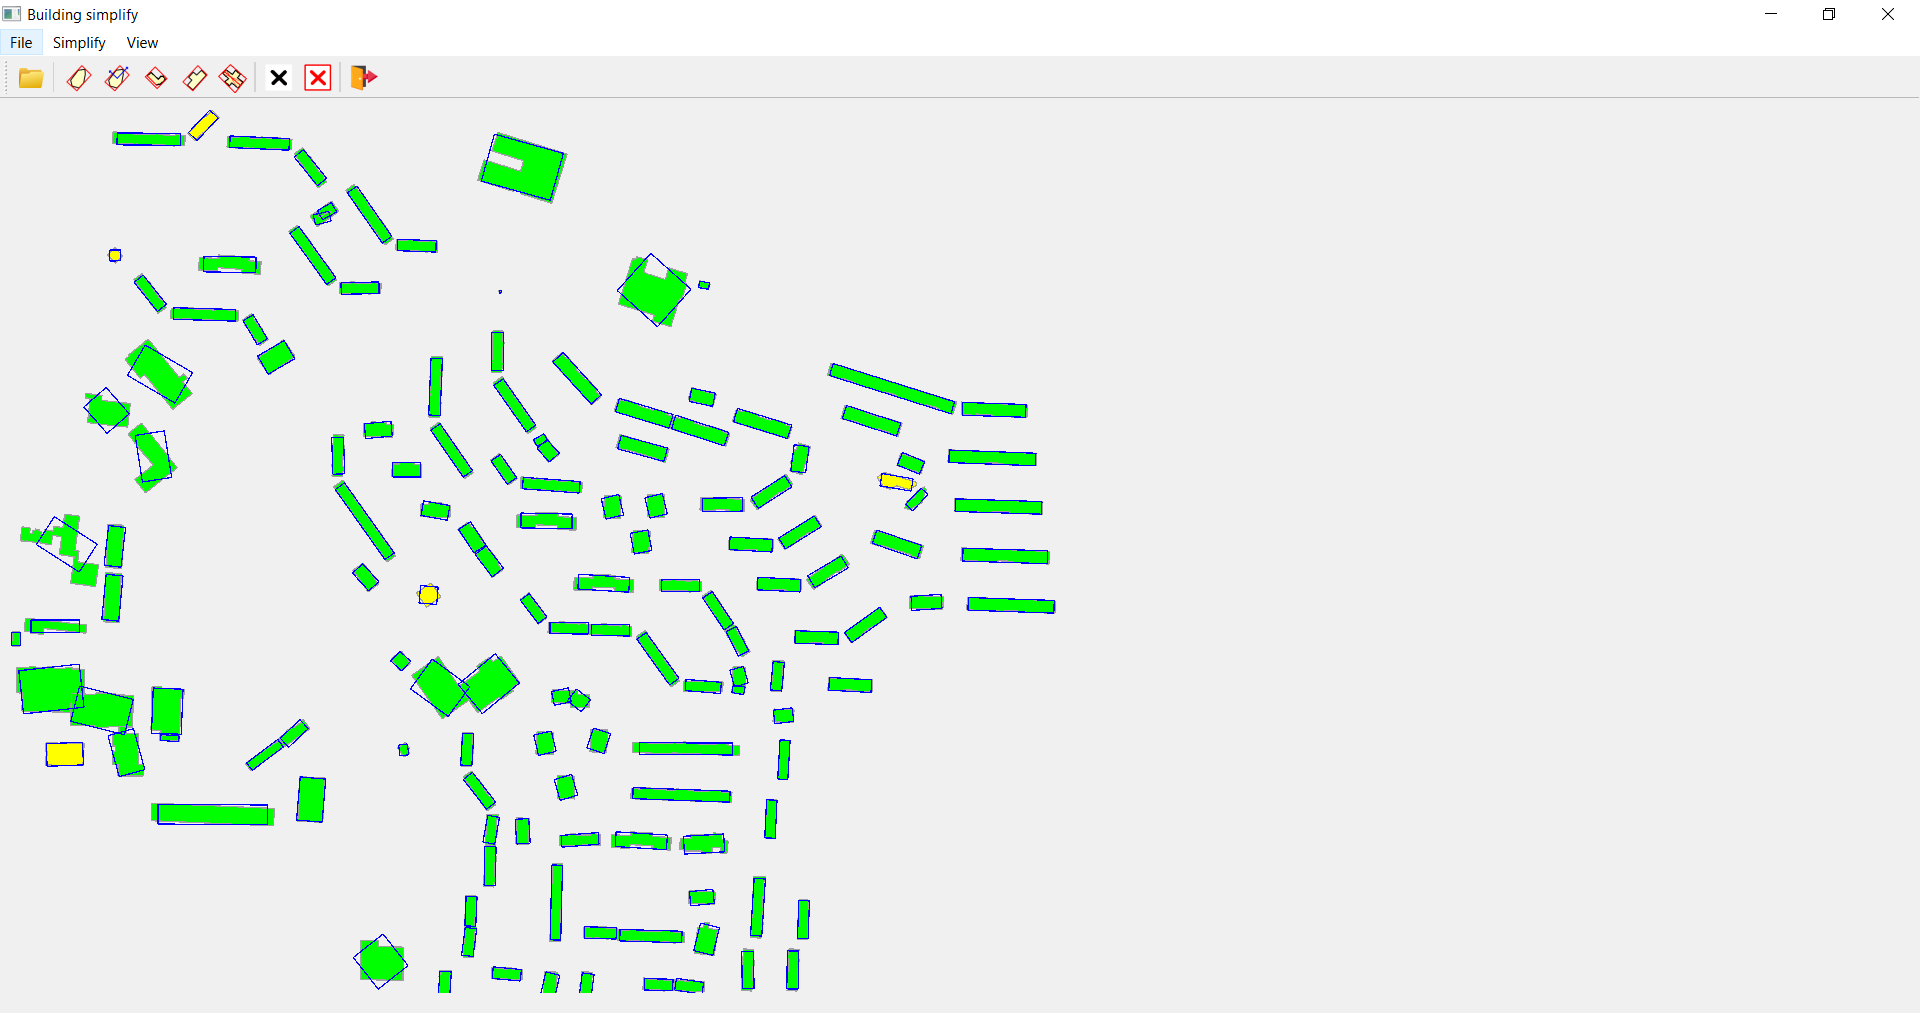
\includegraphics[width=1\linewidth]{app1.png}
    \caption{Ukázka vykreslení generalizovaných budov v aplikaci}
    \label{fig:app_preview}
\end{figure}

\subsection{Aplikace}

Aplikace je vytvořena v jazyce Python s využitím knihoven \texttt{PyQt6}. Po spuštění může uživatel nahrát shapefile, který se vykreslí do okna aplikace. Následně lze spustit generalizaci podle zvolené metody – MAER, PCA, Longest Edge, Wall Average nebo Weighted Bisector – a sledovat její výsledek v porovnání s původními daty.

Ovládací ikony v horní části aplikace slouží pro načtení souboru, spuštění algoritmu, vymazání dat nebo ukončení aplikace.

\begin{figure}[H]
    \centering
    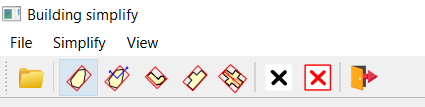
\includegraphics[width=0.5\linewidth]{app2.png}
    \caption{Ovládací prvky aplikace}
    \label{fig:gui_overview}
\end{figure}

Uživatel tak získává nástroj pro interaktivní porovnání výsledků jednotlivých metod generalizace nad reálnými prostorovými daty.

\section{Třídy a metody tříd}

Pro implementaci aplikace byly využity čtyři základní části: hlavní uživatelské rozhraní (`MainForm`), vykreslovací komponenta (`Draw`), třída obsahující výpočetní algoritmy (`Algorithms`) a pomocný skript pro načítání shapefilů (`read\_shp.py`). Níže jsou stručně popsány jejich funkce a hlavní metody.

\subsection{Třída MainForm}
Třída \texttt{MainForm} obsahuje veškerou logiku pro hlavní okno aplikace, nastavuje menu a nástrojovou lištu a propojuje kliknutí uživatele s odpovídajícími metodami z třídy \texttt{Algorithms}. Hlavní metody jsou:

\begin{itemize}
    \item \textbf{setupUi, retranslateUi} – vytvoření a překlad uživatelského rozhraní (tlačítka, ikony, menu).
    \item \textbf{openFileDialog} – otevření dialogového okna pro výběr \texttt{.shp} souboru. Po načtení volá \texttt{load\_shapefile} a vykresluje načtené polygony do \texttt{Canvas}.
    \item \textbf{simplifyBuildingMBR} – volá metodu \texttt{createMBR} ze třídy \texttt{Algorithms} pro všechny budovy v aplikaci a výsledek vykreslí.
    \item \textbf{simplifyBuildingPCA} – podobně volá \texttt{createBRPCA}.
    \item \textbf{simplifyBuildingLongestEdge} – spouští \texttt{createLongestEdge}.
    \item \textbf{simplifyBuildingWallAverage} – spouští \texttt{createWallAverage}.
    \item \textbf{simplifyBuildingWeightedBisector} – spouští \texttt{createWeightedBisector}.
    \item \textbf{clearData} – vymaže z widgetu \texttt{Canvas} všechny načtené budovy.
    \item \textbf{clearResult} – vymaže z widgetu \texttt{Canvas} pouze výsledné generalizované obdélníky (původní budovy zůstávají).
    \item \textbf{closeApp} – ukončí aplikaci.
\end{itemize}

Všechny metody generalizace mají podobnou strukturu: načtou polygonové objekty z \texttt{Canvas}, zavolají odpovídající algoritmus, uloží výsledek zpět do \texttt{Canvas} a vyvolají překreslení okna voláním \texttt{repaint()}. Tím je zajištěno, že uživatel okamžitě vidí výsledek.

\subsection{Třída Draw}
Třída \texttt{Draw} zajišťuje samotné vykreslování půdorysů budov (původních i generalizovaných) ve vykreslovacím okně. Dále obsahuje funkce pro mazání vykreslených dat. Udržuje tři seznamy: 
\begin{itemize}
    \item \texttt{self.buildings} – obsahuje originální načtené polygony budov,
    \item \texttt{self.buildings\_simp} – obsahuje generalizované obdélníky získané z aplikovaných metod,
    \item \texttt{self.building\_correct} – obsahuje polygonové objekty, u kterých generalizace proběhla úspěšně dle zvolených kritérií.
\end{itemize}

Metody této třídy zahrnují:
\begin{itemize}
    \item \textbf{paintEvent(e)} – hlavní vykreslovací metoda. Nejprve vykreslí původné budovy pomocí žluté výplně a šedých kontur. Následně vykreslí objekty z \texttt{building\_correct} se zelenou výplní a nakonec vykreslí generalizované obdélníky (obsah \texttt{buildings\_simp}) modrou konturou a průhlednou výplní.
    \item \textbf{paintInputEvent(polygons)} – načte a uloží polygony do seznamu \texttt{self.buildings}.
    \item \textbf{setSimplifiedBuilding(building\_simp\_)} – nastaví generalizovaný polygon (nebo polygony) do seznamu \texttt{self.buildings\_simp}.
    \item \textbf{clearBuildings()} – vymaže všechny objekty a překreslí obrazovku.
    \item \textbf{clearSimpBuilding()} – vymaže pouze výsledné generalizované obdélníky, původní budovy zůstávají zobrazeny.
\end{itemize}

\subsection{Třída Algorithms}
Obsahuje veškeré algoritmy pro generalizaci budov, práci s polygonem a prostorové analýzy. Principy jednotlivých algoritmů jsou popsány v kapitolách výše.

\begin{itemize}
    \item \textbf{createCH} – vytvoření konvexní obálky (Jarvis Scan).
    \item \textbf{createMMB} – výpočet minmax boxu.
    \item \textbf{rotate} – otočení polygonu o zadaný úhel.
    \item \textbf{resizeRectangle} – úprava rozměrů obdélníku tak, aby odpovídal ploše zadaného polygonu.
    \item \textbf{createMBR} – generalizace pomocí Minimum Area Enclosing Rectangle.
    \item \textbf{createBRPCA} – generalizace pomocí PCA.
    \item \textbf{createLongestEdge} – generalizace metodou Longest Edge.
    \item \textbf{createWallAverage} – generalizace metodou Wall Average.
    \item \textbf{createWeightedBisector} – generalizace metodou Weighted Bisector.
    \item \textbf{gain} – výpočet směrnice hrany - varcí úhel.
    \item \textbf{checkForIntersection} – vrací informaci o tom, zda úsečka protíná některou hranu polygonu.
    \item \textbf{euclideanDistance} – výpočet eukleidovské vzdálenosti mezi dvěma body.
    \item \textbf{evaluateSimplification} – vyhodnocuje úspěšnost identifikace hlavního směru budovy. 
\end{itemize}

\subsection{Soubor \texttt{read\_shp.py}}
Skript obsahuje funkci pro načítání shapefile souborů pomocí knihovny GeoPandas. Geometrie jsou převedeny na vykreslitelný formát \texttt{QPolygonF} a přeškálovány pro velikost aplikačního okna.

\section{Hodnocení úspěšnosti detekce hlavních směrů}

Pro hodnocení úspěšnosti detekce hlavních směrů byly vybrány tři datasety, každý reprezentující jiný typ zástavby. První obsahoval vesnickou izolovanou zástavbu rodinných domů (část KÚ Žizníkov u České Lípy), druhý obsahoval největší českolipské sídliště Špičák s převládajícími podlouhlými panelovými domy. Třetí dataset zahrnul historickou zástavbu centra České Lípy v ulicích kolem náměstí T. G. Masaryka.

Pro hodnocení efektivity detekce hlavních směrů byla zvolena metoda založená na výpočtu střední hodnoty čtverců úhlových odchylek jednotlivých segmentů objektů dle vzorce z \parencite{bayer_prednaska}:

\[
\Delta\sigma = \frac{\pi}{2n}\sqrt{\sum_{i=1}^{n}(r_{i}-r)^{2}}
\]


Podle výsledků uvedených v tabulce 2 dosáhly generalizační metody u rodinných domů podobných úspěšností. Nejvyšší míru úspěšnosti zaznamenala metoda MBR, která dosáhla 93,9\,\%, čímž se ukázala jako nejefektivnější přístup při zjednodušování půdorysů budov na daném datasetu. Naopak metoda Weighted Bisector vykázala nejnižší úspěšnost, dosahující pouze 83,8\,\%. Podrobné výsledky jednotlivých metod jsou uvedeny v tabulce níže.

\begin{table}[H]
\centering
\begin{tabular}{lrrr}
\hline
\textbf{Metoda} & \textbf{Budov} & \textbf{OK} & \textbf{Úspěšnost [\%]} \\
\hline
Metoda MBR            & 148 & 139 & 93.9 \\
Metoda PCA            & 148 & 130 & 87.8 \\
Metoda Longest Edge   & 148 & 138 & 93.2 \\
Metoda Wall Average   & 148 & 138 & 93.2 \\
Metoda Weighted Bisector & 148 & 124 & 83.8 \\
\hline
\end{tabular}
\caption{Úspěšnost generalizace - Rodinné domy}
\label{tab:generalization_family_houses}
\end{table}

V případě sídlištní zástavby dosahují metody MBR, Longest Edge a Wall Average téměř perfektní úspěšnosti (98,6\,\%), což potvrzuje jejich schopnost přesně zachytit pravidelné geometrické tvary budov. Metoda PCA vykazuje úspěšnost 95,8\,\% a Metoda Weighted Bisector má mírně nižší úspěšnost 95,1\,\%. Podrobné výsledky jednotlivých metod jsou shrnuty v tabulce 3 níže.

\begin{table}[H]
\centering
\begin{tabular}{lrrr}
\hline
\textbf{Metoda} & \textbf{Budov} & \textbf{OK} & \textbf{Úspěšnost [\%]} \\
\hline
Metoda MBR            & 144 & 142 & 98.6 \\
Metoda PCA            & 144 & 138 & 95.8 \\
Metoda Longest Edge   & 144 & 142 & 98.6 \\
Metoda Wall Average   & 144 & 142 & 98.6 \\
Metoda Weighted Bisector & 144 & 137 & 95.1 \\
\hline
\end{tabular}
\caption{Úspěšnost generalizace - Sídliště Špičák}
\label{tab:generalization_spicak}
\end{table}

Dataset historického centra města Česká Lípa obsahuje 360 budov s výrazně komplikovanějšími a nepravidelnými půdorysy. U těchto budov dosahují metody generalizace nižších úspěšností než v případě modernější, pravidelnějších zástavby. Nejvyšší úspěšnost zaznamenala Metoda Wall Average (90.3\,\%), následovaná Metodou Longest Edge (90.0\,\%). U historických budov s komplikovanými tvary mají všechny metody častěji problémy s přesným zachycením základní orientace. Podrobné výsledky jednotlivých metod jsou shrnuty v tabulce 4.

\begin{table}[H]
\centering
\begin{tabular}{lrrr}
\hline
\textbf{Metoda} & \textbf{Budov} & \textbf{OK} & \textbf{Úspěšnost [\%]} \\
\hline
Metoda MBR            & 360 & 322 & 89.4 \\
Metoda PCA            & 360 & 301 & 83.6 \\
Metoda Longest Edge   & 360 & 324 & 90.0 \\
Metoda Wall Average   & 360 & 325 & 90.3 \\
Metoda Weighted Bisector & 360 & 291 & 80.8 \\
\hline
\end{tabular}
\caption{Úspěšnost generalizace - Historické centrum}
\label{tab:generalization_historic_center}
\end{table}

Výsledky testování generalizace ukazují, že u moderních a relativně pravidelných budov, jako je zástavba rodinných domů poskytují metody Minimum Area Enclosing Rectangle, Longest Edge a Wall Average velmi vhodné aproximace s úspěšností kolem 93–94\,\%, zatímco PCA a zejména Weighted Bisector vykazují o něco nižší úspěšnost (87,8\,\% až 83,8\,\%). Na moderním sídlišti Špičák dosahují všechny metody ještě vyšších hodnot – s MBR, Longest Edge a Wall Average téměř 98,6\,\% úspěšností, což poukazuje na jejich schopnost přesně zachytit jednotný tvar budov. Naproti tomu v historickém centru, kde jsou budovy výrazně nepravidelnější a geometrie komplexnější, jsou celkové úspěšnosti metod nižší (od 80,8\,\% u Weighted Bisector do 90,3\,\% u Wall Average). Lze říci, že zvolená algoritmická řešení poskytují optimální aproximaci pro pravidelnou zástavbu, zatímco u historických, komplikovanějších půdorysů dochází ke snížení přesnosti.

\section{Závěr}
V rámci této úlohy byla vytvořena aplikace, která umožňuje generalizaci budov do úrovně LOD0. Bylo implementováno pět metod určování hlavních směrů: Minimum Area Enclosing Rectangle, PCA, Longest Edge, Wall Average a Weighted Bisector. Každá z nich nabízí jinou heuristiku pro nalezení hlavního směru polygonu, což se odráží ve tvaru a natočení výsledného obdélníku.

Import dat je omezen na soubory ve formátu \texttt{.shp}, do budoucna by mohlo být zajímavé rozšířit podporu i pro jiné formáty (např. GeoJSON). Vhodným vylepšením by byla také možnost interaktivního přibližování a posouvání zobrazených polygonů.

Bylo také provedeno vyhodnocení úspěšnosti detekce hlavních směrů různými metody nad různými typy zástavby.

Kód aplikace je připraven tak, aby jej bylo možné rozšiřovat o další metody generalizace nebo různé vizualizační funkce. Díky přehledné struktuře \texttt{MainForm}, \texttt{Draw} a \texttt{Algorithms} je možné snadno přidávat nové funkcionality a experimentovat s dalšími přístupy k zjednodušování půdorysů budov.

Program je volně dostupný na adrese \href{https://github.com/aktaz-fesoj/building_generalization}{https://github.com/aktaz-fesoj/building\_generalization}.

\printbibliography[title={Zdroje}]



\end{document}